\chapter{Introduction}
Des atomes aux galaxies, jusqu'à l'univers dans son ensemble, tous les objets autour de nous peuvent être considérés en mouvement. Dans l'étude du monde qui nous entoure, il s'agit d'un des premiers aspects auquel l'homme s'est intéressé. L'étude scientifique du mouvement a commencé avec Galilée (1564-1642) puis Newton (1642-1727). Le mouvement de corps comme une galaxie avec les étoiles qui la composent ou celui des molécules d'air dans le vent sont hautement complexes mais d'autre comme celui d'un objet en chute libre ou d'une voiture sur une autoroute sont plus simples.
La \motcle{cinématique} est l'étude des mouvements. Dans le cadre de ce cours, seuls les mouvements les plus simples seront abordés : les mouvements continus en ligne droite puis, plus tard, les mouvements circulaires.
\begin{figure}[!ht]
    \centering
    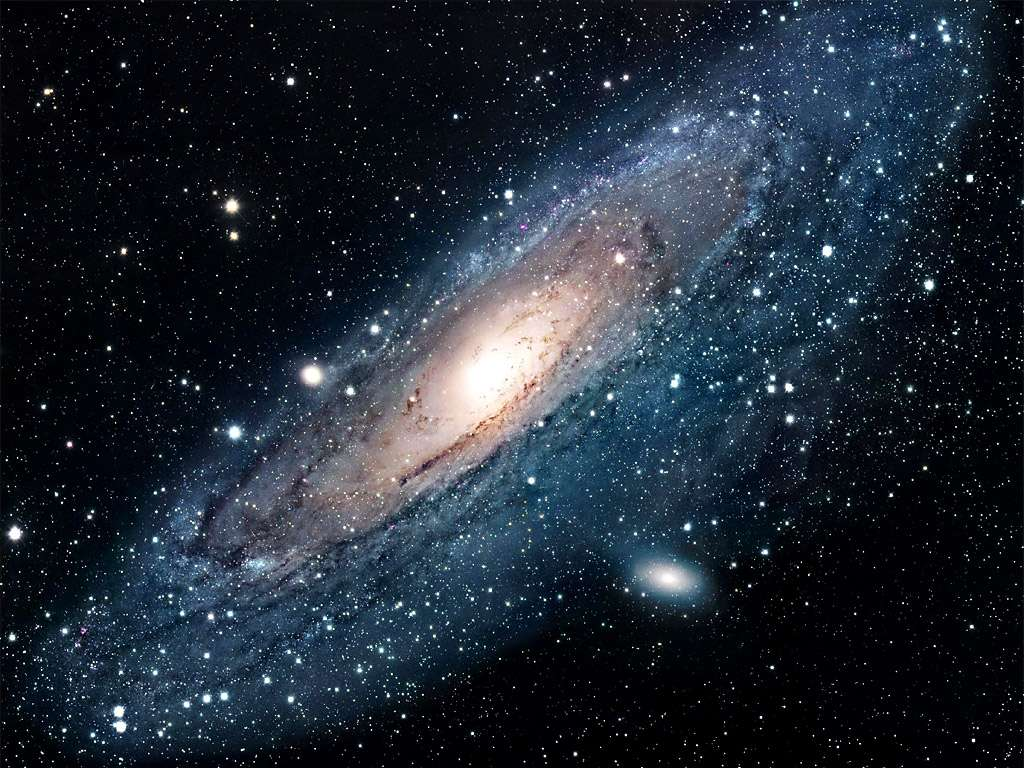
\includegraphics[width=0.5\linewidth]{galaxie_andromede.png}
    \caption{La galaxie d'Andromède, la galaxie la plus proche de la Voie lactée. }
    \label{galaxie_andromede}
\end{figure}


\chapter{Notions de base}
\section{Mobile et point matériel}
Quelle que soit la complexité du corps dont on cherche à étudier le mouvement, le \motcle{mobile}, celui-ci sera représenté par un point ou quelque chose de suffisamment petit par rapport au déplacement effectué. Lorsque le mobile est complexe mais qu'il s'agit d'un solide non déformable, il existe toujours un point appelé \motcle{centre de masse} ou centre d'inertie qui se comporte comme si toute la masse du corps était située en ce point.
\begin{figure}[!ht]
    \centering
    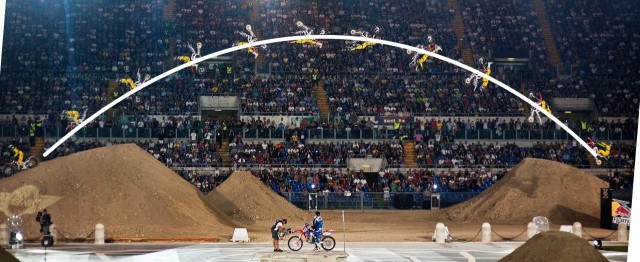
\includegraphics[width=0.7\linewidth]{mouvement_centre_masse.png}
    \caption{Le centre de masse décrit une parabole (Centre of mass in extreme sports). }
    \label{mouvement_centre_masse}
\end{figure}

\newpage

\section{Référentiel}
Pour décrire un mouvement de manière quantitative il faut pouvoir localiser le mobile dans l'espace et dans le temps. Notre espace étant à trois dimensions, trois axes de référence sont nécessaires. Pour d'évidentes questions de facilité, ces axes seront presque toujours perpendiculaires entre-eux et avec des graduations linéaires. Les systèmes que nous étudierons seront également munis d'une horloge ou d'un chronomètre.

\begin{encadre}
    \motcle{Référentiel} ou système de référence : ensemble d'axes gradués souvent perpendiculaires entre eux (repère cartésien et orthonormé) qui permettent de situer le mobile dans l'espace.
\end{encadre}

Pour l'étude des mouvements rectilignes, un référentiel réduit à un seul axe est suffisant. Le référentiel terrestre constitue souvent un système de référence privilégié.
On pourra dire qu'un objet est en mouvement lorsque sa position dans le référentiel varie entre deux instants.

\section{Relativité du mouvement}
On considère qu'un corps est en mouvement si la distance qui le sépare d'un ou plusieurs points varie au cours du temps. La notion de mouvement est relative, elle dépend du référentiel choisi. Le plus souvent, la surface de la Terre sera choisie comme référentiel mais il faut toujours être conscient du référentiel sur base duquel un mouvement est étudié.
Par exemples :
\begin{itemize}[label= \textbullet]
    \item Une personne est assise dans un train, ce train se déplace sur les rails. Cette personne est au repos par rapport au train mais est en mouvement par rapport à un arbre situé au bord des voies. On peut aussi dire que l'arbre est en mouvement si le train est choisi comme référentiel.
    \item Une personne marche à contre sens sur un escalator de façon à rester sur place par rapport à l'escalier se trouvant à côté de l'escalator. Est-elle en mouvement ou au repos?
\end{itemize}

\newpage

\section{Position}
Le schéma ci-dessous représente un homme qui cours, la ligne graduée sert de référentiel. La position du mobile dépend du temps, elle est une fonction du temps. Il existe deux façons de noter la position du mobile,
\begin{itemize}[label= \textbullet]
    \item soit on fait référence au fait que la position est fonction du temps et celle-ci se note \(x(t)\)
    \item soit on met en évidence de numéro de la mesure et la position se note \(x_i\).
\end{itemize}

\begin{figure}[!ht]
    \centering
    \resizebox{.7\linewidth}{!}{

\newcommand{\bonhommec}{
\begin{scope}[xshift=-3.5pt]%on décale pour que le bonhomme soit aligné par rapport à son milieu
\draw [fill=black,draw=none,line width=0.1pt] (2.7pt,9.9pt)
-- (0.2pt,7.4pt)
-- (1.0pt,6.7pt)
-- (3.1pt,8.8pt)
-- (5.0pt,8.8pt)
-- (2.4pt,6.1pt)
-- (2.4pt,3.7pt)
-- (0.0pt,3.7pt)
-- (0.0pt,2.7pt)
-- (3.5pt,2.7pt)
-- (3.5pt,5.0pt)
-- (5.8pt,2.7pt)
-- (5.8pt,0.0pt)
-- (6.9pt,0.0pt)
-- (6.9pt,3.1pt)
-- (4.7pt,5.4pt)
-- (6.6pt,7.3pt)
-- (6.6pt,4.9pt)
-- ++(3.5pt,0.0pt)
-- ++(0.0pt,1.1pt)
-- ++(-2.4pt,0.0pt)
-- ++(0.0pt,2.4pt)
-- ++(-1.5pt,1.5pt)
-- cycle
;
\draw [fill=black,draw=none,line width=0.1pt] (8pt,10pt) circle (1.2pt);
\end{scope}
}

\newcommand{\bonhommer}{
\draw [fill=black,draw=none,line width=0.3pt,xshift=-15] (0.0pt,44.4pt)
-- (0.0pt,22.9pt)
-- (5.8pt,22.9pt)
-- (5.8pt,38.7pt)
-- (7.0pt,38.7pt)
-- (7.0pt,0.0pt)
-- ++(5.7pt,0.0pt)
-- ++(0.0pt,18.0pt)
-- ++(3.1pt,0.0pt)
-- (15.8pt,0.0pt)
-- ++(5.7pt,0.0pt)
-- ++(0.0pt,38.7pt)
-- ++(1.2pt,0.0pt)
-- (22.7pt,22.9pt)
-- ++(5.7pt,0.0pt)
-- ++(0.0pt,21.5pt)
-- cycle
;
\begin{scope}[xscale=1,yscale=-1,xshift=-15]
\draw [fill=black,draw=none,line width=0.3pt] (14.2pt,-53.4pt) circle (6.6pt);
\end{scope}
}

\begin{tikzpicture}

\tikzset{>=latex}

\def\tkzCoeffSubColor{20} 
\def\tkzCoeffSubLw{0.2}

\tkzInit[xmin=0,xmax=10,xstep=1]
\tkzAxeX
\tkzText(0,1){\footnotesize{2[s]}}
\tkzText(2,1){\footnotesize{3[s]}}
\tkzText(6,1){\footnotesize{5[s]}}

\begin{scope}[shift={(2,0)},scale=1.8]
\bonhommec
\end{scope}

\begin{scope}[shift={(6,0)},scale=1.8]
\bonhommec
\end{scope}

\begin{scope}[scale=.35]
\bonhommer
\end{scope}

%\node [anchor=base] at (0,0){\includegraphics[height=1.5\baselineskip]{./images/bonhomme_repos.pdf}};
\end{tikzpicture}
}
    \caption{Un mouvement à une dimension.}
    \label{position_referentiel_1}
\end{figure}

Complète le tableau ci-dessous en attribuant un symbole à chaque valeur de temps et de position.\\
\renewcommand{\arraystretch}{1.5}
\begin{tabularx}{\linewidth}{|X|X|X|X|X|}
    \hline
    \multicolumn{2}{|l|}{Temps[s]} & \multicolumn{3}{l|}{Position [m]}                              \\
    \hline
    Symbole                        & Valeur                            & Symbole & Symbole & Valeur \\
    \hline
                                   &                                   &         &         &        \\
    \hline
                                   &                                   &         &         &        \\
    \hline
                                   &                                   &         &         &        \\
    \hline
\end{tabularx}
\renewcommand{\arraystretch}{1}\\



\begin{encadre}
    La première valeur de temps se note \(t_0\). La position à l'instant \(t_0\) se note \(x_0\). Attention, \(x_0\) ne vaut pas forcément zéro et \(t_0\) non plus.
\end{encadre}

\newpage

\section{Trajectoire}
La trajectoire d'un objet en mouvement est l'ensemble des positions qu'a occupé cet objet au cours de son mouvement.

\begin{figure}[!ht]
    \centering
    \resizebox{.6\linewidth}{!}{

\newcommand{\halfwing}[1]{
	\begin{scope}[yscale=1,xscale=#1]
		% Lower Wing
		\filldraw[fill=black!90!white!,draw=black,ultra thin,rounded corners=0.05mm] (0,0.2) -- (0,1.4) -- (-2,1.4) .. controls (-4,0.8) .. (-4.3,0.2) .. controls (-4.48,0.08) .. (-4.5,-0.15) .. controls (-4.9,-0.5) and (-4.9,-0.7) .. (-4.7,-0.9) .. controls (-4.7,-1) .. (-4.6,-1.1) .. controls (-4.9,-1.8) .. (-4.2,-2) -- (-4,-2.4) .. controls (-4.1,-3) .. (-3.6,-3.1) -- (-3.25,-3.7) .. controls (-3.5,-4.5) .. (-4.1,-5.4) .. controls (-4.2,-5.9) and (-3.6,-5.9) .. (-3.5,-5.4) .. controls (-3.55,-5.1) and (-3.4,-4.8) .. (-3,-4.1) -- (-2.6,-4.1) .. controls (-2.35,-4.35) .. (-2,-4.2) .. controls (-1.75,-4.6) and (-1.25,-4.6) .. (-1.25,-3.90) .. controls (-0.9,-4) .. (-0.6,-2.8) -- (-0.3,-1) -- (0,0.2);
		\shadedraw[top color=blue!45!cyan!,bottom color=blue!20!cyan!,draw=black,rounded corners=0.05mm] (-0.8,-3) .. controls (-0.5,-2) .. (-0.30,-0.95){[rounded corners=0mm] .. controls (-0.15,-0.3) .. (-0.05,0.45) -- (-0.05,0.7)} -- (-0.7,0.4) .. controls (-0.9,-2) .. (-0.8,-3);
		\shadedraw[top color=blue!60!cyan!,bottom color=blue!20!cyan!,draw=black] (-1.1,-2.9) .. controls (-1.4,2) and (0.5,2) .. (-1.1,-2.9);
		\shadedraw[top color=blue!70!cyan!,bottom color=blue!20!cyan!,draw=black] (-1.6,-2.8) .. controls (-0.9,3.7) and (0,-0.1) .. (-1.6,-2.8);
		\shadedraw[top color=blue!70!cyan!,bottom color=blue!20!cyan!,draw=black] (-2.1,-2.6) .. controls (-0.9,3.7) and (-0.3,-0.1) .. (-2.1,-2.6);
		\shadedraw[top color=blue!80!cyan!,bottom color=blue!20!cyan!,draw=black] (-2.6,-2.2) .. controls (-0.3,3.7) and (-0.3,-0.1) .. (-2.6,-2.2);
		\shadedraw[top color=blue!80!cyan!,bottom color=blue!20!cyan!,draw=black] (-3,-1.7) .. controls (0.1,3.7) and (0.1,-0.1) .. (-3,-1.7);
		\shadedraw[top color=blue!80!cyan!,bottom color=blue!20!cyan!,draw=black] (-3.4,-1.2) .. controls (0.77,3) and (0.77,-0.2) .. (-3.4,-1.2);
		\shadedraw[top color=blue!80!cyan!,bottom color=blue!20!cyan!,draw=black] (-3.6,-0.6) .. controls (0.77,2.2) and (0.77,-0.5) .. (-3.6,-0.6);
		\shadedraw[top color=blue!80!cyan!,bottom color=blue!15!cyan!,draw=black] (-3.5,0) .. controls (0.77,1.8) and (0.77,-0.2) .. (-3.5,0);
		\shadedraw[top color=blue!80!cyan!,bottom color=blue!10!cyan!,draw=black] (-2.5,0.7) .. controls (0.77,2) and (0.77,0) .. (-2.5,0.7);
		\shadedraw[top color=blue!45!cyan!,bottom color=blue!15!cyan!,draw=black] (-0.05,0.6) -- (-0.05,0.9) .. controls (-4,-0.5) and (-1.5,-2) .. (-0.05,0.6);

		% Upper Wing
		\filldraw[fill=black!90!white!,draw=black,ultra thin] (0,1) -- (0,2.2) [rounded corners=0.05mm] parabola[bend at end] (-6,6) -- (-5,1) -- (0,1);
		\shadedraw[top color=blue!20!cyan!,bottom color=blue!70!cyan!,draw=black] (-4,3.5) .. controls (3,-1) and (-2,4) .. (-4,3.5);
		\shadedraw[top color=blue!15!cyan!,bottom color=blue,draw=black] (-4.1,3) .. controls (3.9,-0.5) and (-2.1,4) .. (-4.1,3);
		\shadedraw[top color=blue!15!cyan!,bottom color=blue!80!cyan!,draw=black] (-4.2,2.5) .. controls (4,-0.2) and (-2.2,3.5) .. (-4.2,2.5);
		\shadedraw[top color=blue!15!cyan!,bottom color=blue!70!cyan!,draw=black] (-4.2,1.8) .. controls (4,0.3) and (-2.2,3) .. (-4.2,1.8);
		\shadedraw[top color=cyan,bottom color=blue!60!cyan!,draw=black] (-4.2,1.2) .. controls (4.05,0.9) and (-2.2,2.4) .. (-4.2,1.2);
		\shadedraw[top color=cyan,bottom color=blue!60!cyan!,draw=black] (-0.05,1.85) -- (-0.05,1.80) .. controls (-6.5,6.5) and (-2,5.5) .. (-0.05,1.85);
		\shadedraw[top color=blue!10!cyan!,bottom color=blue!50!cyan!,draw=black] (-0.05,1.8) -- (-0.05,1.4) .. controls (-7.5,5.5) and (-2,5) .. (-0.05,1.8);
	\end{scope}
}%fin de halfwing

\newcommand{\antenna}
{\draw[ultra thin] (0,2.7) parabola[bend at end] (-1.5,5.2);
	\filldraw[fill=black!80!white!,draw=black,ultra thin] (-1.5,5.2) .. controls ++(-0.2,0.1) and ++(-0.5,-0.3) .. ++(0,0);
	\begin{scope}[yscale=1,xscale=-1]
		\draw[ultra thin] (0,2.7) parabola[bend at end] (-1.5,5.2);
		\filldraw[fill=black!80!white!,draw=black,ultra thin] (-1.5,5.2) .. controls ++(-0.2,0.1) and ++(-0.5,-0.3) .. ++(0,0);
	\end{scope}
}

\newcommand{\body}
{\filldraw[fill=black!80!white!,draw=black,ultra thin,rounded corners=0.05mm] (0,2.5) -- (0.35,2.5) -- (0.45,1.5) -- (0.45,0) -- (0.25,-2) -- (-0.25,-2) -- (-0.45,0) -- (-0.45,1.5) -- (-0.35,2.5) -- (0,2.5);
	\shade[inner color=black!70!white!,outer color=black!80!white!] (0,2.24) ellipse (0.35cm and 0.24cm);
	\shade[inner color=black!70!white!,outer color=black!80!white!] (0,1.75) ellipse (0.4cm and 0.25cm);
	\shade[inner color=black!70!white!,outer color=black!80!white!] (0,1.25) ellipse (0.42cm and 0.25cm);
	\shade[inner color=black!70!white!,outer color=black!80!white!] (0,0.75) ellipse (0.42cm and 0.25cm);
	\shade[inner color=black!70!white!,outer color=black!80!white!] (0,0.25) ellipse (0.42cm and 0.25cm);
	\shade[inner color=black!70!white!,outer color=black!80!white!] (0,-0.25) ellipse (0.4cm and 0.25cm);
	\shade[inner color=black!70!white!,outer color=black!80!white!] (0,-0.75) ellipse (0.35cm and 0.25cm);
	\shade[inner color=black!70!white!,outer color=black!80!white!] (0,-1.25) ellipse (0.3cm and 0.25cm);
	\shade[inner color=black!70!white!,outer color=black!80!white!] (0,-1.74) ellipse (0.25cm and 0.24cm);
}

\newcommand{\head}
{
	\shadedraw[inner color=black!60!white!,outer color=black!80!white!,draw=black,ultra thin,rounded corners=0.05mm] (0,3) -- (0.45,3) -- (0.2,2.3) -- (-0.2,2.3) -- (-0.45,3) -- (0,3);
	\shadedraw[inner color=white!60!black,outer color=black, draw=black,ultra thin] (-0.25,2.85) circle (0.2cm);
	\shadedraw[inner color=white!60!black,outer color=black, draw=black,ultra thin] (0.25,2.85) circle (0.2cm);
}

\newcommand{\butterfly}{
	\halfwing{1}
	\halfwing{-1}
	\antenna
	\body
	\head
}%fin de butterfly 



\begin{tikzpicture}

\draw [fill=none,draw=red,line width=0.5,dashed] (0,0)
.. controls ++(-0.02,.64) and ++(-.64,-.22) .. (1,1.5)
.. controls ++(.91,.32) and ++(-1.21,0.06) .. (4,-.5)
.. controls ++(.79,-0.02) and ++(-.41,-.65) .. (6,1.5)
.. controls ++(.23,.37) and ++(.29,-.37) .. (6,3)
.. controls ++(-.25,.33) and ++(-0.05,.5) .. (5,3)
.. controls ++(0.05,-.51) and ++(-.46,0.01) .. (6,2)
.. controls ++(1.09,-0.03) and ++(.56,-1.13) .. (9,4)
.. controls ++(-.49,.71) and ++(.35,-.76) .. (7,5)
;
\begin{scope}[shift={(7,5)},rotate=-30,scale=.1]
\butterfly
\end{scope}
\end{tikzpicture}
}
    \caption{La trajectoire,en rouge, dans un mouvement à deux dimensions.}
    \label{position_referentiel_2}
\end{figure}

\section{Le déplacement et la durée}
Au cours de son mouvement, le mobile passe par une série de positions. Le \motcle{déplacement}, correspond à la différence entre 2 positions.
Pour calculer un déplacement, on fait la différence entre la deuxième et la première position : \(\Delta x=x_2-x_1\) (pour un mouvement à une dimension, sinon, on écrirait \(\Delta r=r_2-r_1\)).

La \motcle{durée} mesure le temps qui s'est écoulé entre ces deux observations, elle correspond à la différence de temps entre celles-ci. Durée  :\(\Delta t=t_2-t_1\).

\begin{figure}[!ht]
    \centering
    \resizebox{.6\linewidth}{!}{

\newcommand{\halfwing}[1]{
	\begin{scope}[yscale=1,xscale=#1]
		% Lower Wing
		\filldraw[fill=black!90!white!,draw=black,ultra thin,rounded corners=0.05mm] (0,0.2) -- (0,1.4) -- (-2,1.4) .. controls (-4,0.8) .. (-4.3,0.2) .. controls (-4.48,0.08) .. (-4.5,-0.15) .. controls (-4.9,-0.5) and (-4.9,-0.7) .. (-4.7,-0.9) .. controls (-4.7,-1) .. (-4.6,-1.1) .. controls (-4.9,-1.8) .. (-4.2,-2) -- (-4,-2.4) .. controls (-4.1,-3) .. (-3.6,-3.1) -- (-3.25,-3.7) .. controls (-3.5,-4.5) .. (-4.1,-5.4) .. controls (-4.2,-5.9) and (-3.6,-5.9) .. (-3.5,-5.4) .. controls (-3.55,-5.1) and (-3.4,-4.8) .. (-3,-4.1) -- (-2.6,-4.1) .. controls (-2.35,-4.35) .. (-2,-4.2) .. controls (-1.75,-4.6) and (-1.25,-4.6) .. (-1.25,-3.90) .. controls (-0.9,-4) .. (-0.6,-2.8) -- (-0.3,-1) -- (0,0.2);
		\shadedraw[top color=blue!45!cyan!,bottom color=blue!20!cyan!,draw=black,rounded corners=0.05mm] (-0.8,-3) .. controls (-0.5,-2) .. (-0.30,-0.95){[rounded corners=0mm] .. controls (-0.15,-0.3) .. (-0.05,0.45) -- (-0.05,0.7)} -- (-0.7,0.4) .. controls (-0.9,-2) .. (-0.8,-3);
		\shadedraw[top color=blue!60!cyan!,bottom color=blue!20!cyan!,draw=black] (-1.1,-2.9) .. controls (-1.4,2) and (0.5,2) .. (-1.1,-2.9);
		\shadedraw[top color=blue!70!cyan!,bottom color=blue!20!cyan!,draw=black] (-1.6,-2.8) .. controls (-0.9,3.7) and (0,-0.1) .. (-1.6,-2.8);
		\shadedraw[top color=blue!70!cyan!,bottom color=blue!20!cyan!,draw=black] (-2.1,-2.6) .. controls (-0.9,3.7) and (-0.3,-0.1) .. (-2.1,-2.6);
		\shadedraw[top color=blue!80!cyan!,bottom color=blue!20!cyan!,draw=black] (-2.6,-2.2) .. controls (-0.3,3.7) and (-0.3,-0.1) .. (-2.6,-2.2);
		\shadedraw[top color=blue!80!cyan!,bottom color=blue!20!cyan!,draw=black] (-3,-1.7) .. controls (0.1,3.7) and (0.1,-0.1) .. (-3,-1.7);
		\shadedraw[top color=blue!80!cyan!,bottom color=blue!20!cyan!,draw=black] (-3.4,-1.2) .. controls (0.77,3) and (0.77,-0.2) .. (-3.4,-1.2);
		\shadedraw[top color=blue!80!cyan!,bottom color=blue!20!cyan!,draw=black] (-3.6,-0.6) .. controls (0.77,2.2) and (0.77,-0.5) .. (-3.6,-0.6);
		\shadedraw[top color=blue!80!cyan!,bottom color=blue!15!cyan!,draw=black] (-3.5,0) .. controls (0.77,1.8) and (0.77,-0.2) .. (-3.5,0);
		\shadedraw[top color=blue!80!cyan!,bottom color=blue!10!cyan!,draw=black] (-2.5,0.7) .. controls (0.77,2) and (0.77,0) .. (-2.5,0.7);
		\shadedraw[top color=blue!45!cyan!,bottom color=blue!15!cyan!,draw=black] (-0.05,0.6) -- (-0.05,0.9) .. controls (-4,-0.5) and (-1.5,-2) .. (-0.05,0.6);

		% Upper Wing
		\filldraw[fill=black!90!white!,draw=black,ultra thin] (0,1) -- (0,2.2) [rounded corners=0.05mm] parabola[bend at end] (-6,6) -- (-5,1) -- (0,1);
		\shadedraw[top color=blue!20!cyan!,bottom color=blue!70!cyan!,draw=black] (-4,3.5) .. controls (3,-1) and (-2,4) .. (-4,3.5);
		\shadedraw[top color=blue!15!cyan!,bottom color=blue,draw=black] (-4.1,3) .. controls (3.9,-0.5) and (-2.1,4) .. (-4.1,3);
		\shadedraw[top color=blue!15!cyan!,bottom color=blue!80!cyan!,draw=black] (-4.2,2.5) .. controls (4,-0.2) and (-2.2,3.5) .. (-4.2,2.5);
		\shadedraw[top color=blue!15!cyan!,bottom color=blue!70!cyan!,draw=black] (-4.2,1.8) .. controls (4,0.3) and (-2.2,3) .. (-4.2,1.8);
		\shadedraw[top color=cyan,bottom color=blue!60!cyan!,draw=black] (-4.2,1.2) .. controls (4.05,0.9) and (-2.2,2.4) .. (-4.2,1.2);
		\shadedraw[top color=cyan,bottom color=blue!60!cyan!,draw=black] (-0.05,1.85) -- (-0.05,1.80) .. controls (-6.5,6.5) and (-2,5.5) .. (-0.05,1.85);
		\shadedraw[top color=blue!10!cyan!,bottom color=blue!50!cyan!,draw=black] (-0.05,1.8) -- (-0.05,1.4) .. controls (-7.5,5.5) and (-2,5) .. (-0.05,1.8);
	\end{scope}
}%fin de halfwing

\newcommand{\antenna}
{\draw[ultra thin] (0,2.7) parabola[bend at end] (-1.5,5.2);
	\filldraw[fill=black!80!white!,draw=black,ultra thin] (-1.5,5.2) .. controls ++(-0.2,0.1) and ++(-0.5,-0.3) .. ++(0,0);
	\begin{scope}[yscale=1,xscale=-1]
		\draw[ultra thin] (0,2.7) parabola[bend at end] (-1.5,5.2);
		\filldraw[fill=black!80!white!,draw=black,ultra thin] (-1.5,5.2) .. controls ++(-0.2,0.1) and ++(-0.5,-0.3) .. ++(0,0);
	\end{scope}
}

\newcommand{\body}
{\filldraw[fill=black!80!white!,draw=black,ultra thin,rounded corners=0.05mm] (0,2.5) -- (0.35,2.5) -- (0.45,1.5) -- (0.45,0) -- (0.25,-2) -- (-0.25,-2) -- (-0.45,0) -- (-0.45,1.5) -- (-0.35,2.5) -- (0,2.5);
	\shade[inner color=black!70!white!,outer color=black!80!white!] (0,2.24) ellipse (0.35cm and 0.24cm);
	\shade[inner color=black!70!white!,outer color=black!80!white!] (0,1.75) ellipse (0.4cm and 0.25cm);
	\shade[inner color=black!70!white!,outer color=black!80!white!] (0,1.25) ellipse (0.42cm and 0.25cm);
	\shade[inner color=black!70!white!,outer color=black!80!white!] (0,0.75) ellipse (0.42cm and 0.25cm);
	\shade[inner color=black!70!white!,outer color=black!80!white!] (0,0.25) ellipse (0.42cm and 0.25cm);
	\shade[inner color=black!70!white!,outer color=black!80!white!] (0,-0.25) ellipse (0.4cm and 0.25cm);
	\shade[inner color=black!70!white!,outer color=black!80!white!] (0,-0.75) ellipse (0.35cm and 0.25cm);
	\shade[inner color=black!70!white!,outer color=black!80!white!] (0,-1.25) ellipse (0.3cm and 0.25cm);
	\shade[inner color=black!70!white!,outer color=black!80!white!] (0,-1.74) ellipse (0.25cm and 0.24cm);
}

\newcommand{\head}
{
	\shadedraw[inner color=black!60!white!,outer color=black!80!white!,draw=black,ultra thin,rounded corners=0.05mm] (0,3) -- (0.45,3) -- (0.2,2.3) -- (-0.2,2.3) -- (-0.45,3) -- (0,3);
	\shadedraw[inner color=white!60!black,outer color=black, draw=black,ultra thin] (-0.25,2.85) circle (0.2cm);
	\shadedraw[inner color=white!60!black,outer color=black, draw=black,ultra thin] (0.25,2.85) circle (0.2cm);
}

\newcommand{\butterfly}{
	\halfwing{1}
	\halfwing{-1}
	\antenna
	\body
	\head
}%fin de butterfly 



\begin{tikzpicture}
\tikzset{>=latex}
\definecolor{olivegreen}{RGB} {0,125,15}
 
\draw [fill=none,draw=red,line width=0.5,dashed] (0,0)
.. controls ++(-0.02,.64) and ++(-.64,-.22) .. (1,1.5)
.. controls ++(.91,.32) and ++(-1.21,0.06) .. (4,-.5)
.. controls ++(.79,-0.02) and ++(-.41,-.65) .. (6,1.5)
.. controls ++(.23,.37) and ++(.29,-.37) .. (6,3)
.. controls ++(-.25,.33) and ++(-0.05,.5) .. (5,3)
.. controls ++(0.05,-.51) and ++(-.46,0.01) .. (6,2)
.. controls ++(1.09,-0.03) and ++(.56,-1.13) .. (9,4)
.. controls ++(-.49,.71) and ++(.35,-.76) .. (7,5)
;
\begin{scope}[shift={(7,5)},rotate=-30,scale=.1]
\butterfly
\end{scope}

\tkzDefPoints{0/0/O, 7/0/M, 7/5/P, 2/0/N};
\tkzFillAngles[fill=orange](M,O,P)
\tkzDrawPoints[black](O)
\tkzDrawPoints[olivegreen](P)
\tkzLabelPoints[color=black,left=2pt](O)
\tkzLabelPoints[color=olivegreen](P)
\tkzDrawSegment[dim={$L=10[m]$,10pt,above=8pt,rotate=30}](O,P)
\tkzDrawSegment[olivegreen,->](O,P)
\tkzDrawSegment[thin](O,N)

\tkzMarkAngle[mark=solid,-](M,O,P)
\tkzLabelAngle[pos=.5,right=.5](M,O,P){$\alpha=35^{\circ}$}



\end{tikzpicture}
}
    \caption{Le déplacement, en vert, il peut être inférieur à la longueur de la trajectoire.}
    \label{position_referentiel_3}
\end{figure}

\subsection{delta : la différence}
En physique, comme en mathématique, le symbole \(\Delta\) signifie qu'on fait une soustraction entre deux valeurs. On fait toujours cette soustraction entre la valeur \enquote{2} et la valeur \enquote{1}.
\begin{itemize}[label= \textbullet]
    \item \(\Delta x=x_2-x_1\) : c'est un déplacement en ligne droite.
    \item \(\Delta t=t_2-t_1\) : c'est une durée
\end{itemize}


\section{Le vecteur position}
La position d'un objet au sein d'un référentiel peut être représentée par son vecteur position : le vecteur ayant pour origine l'origine du référentiel et son autre extrémité à la position du point. Si l'on note M cette position et O l'origine, le vecteur position se note \(\vec{OM}\) ou \(\vec{r}\).
\begin{figure}[!ht]
    \centering
    \resizebox{0.8\linewidth}{!}{\begin{tikzpicture}
\tikzset{>=latex}
\definecolor{majorgrid_gray}{RGB} {192,192,192}
\definecolor{minorgrid_gray}{RGB} {232,232,232}

\def\tkzCoeffSubColor{20} 
\def\tkzCoeffSubLw{0.2}

\tkzInit[xmax=10,ymax=6,xstep=1,ystep=1]
\tkzGrid[color=majorgrid_gray,line width=0.2mm,sub,subxstep=.5,subystep=.5]

\tkzDrawX[label={$X [m]$},below left=25pt]
\tkzDrawY[label={$Y [m]$},right=5pt]
\tkzAxeXY[label={}] %This macro combines the four macros: \tkzDrawX\tkzDrawY \tkzLabelX\tkzLabelY

\tkzDefPoints{0/0/O, 4/5/M, 7/3/P};
\tkzDrawPoints[black](O)
\tkzDrawPoints[blue](M)
\tkzDrawPoints[red](P)
\tkzLabelPoints[color=black,above=2pt](O)
\tkzLabelPoints[color=blue,above=2pt](M)
\tkzLabelPoints[color=red](P)
\tkzDrawSegment[blue,->](O,M)
\tkzDrawSegment[red,->](O,P)
\tkzLabelSegment[color=blue,above=5pt](O,M){$\vec{OM}$}
\tkzLabelSegment[color=red,above=3pt](O,P){$\vec{OP}$}
\end{tikzpicture}

}
    \caption{Le vecteur position du point M et du point P.}
    \label{vecteur_position}
\end{figure}

\newpage

\section{Le vecteur déplacement}
Le déplacement a été défini comme la différence entre deux positions. Ceci reste valable lorsqu'on considère la dimension vectorielle de la position. Le déplacement de M à P correspond donc à \(\vec{OP} - \vec{OM}\).
\begin{figure}[!ht]
    \centering
    \resizebox{0.8\linewidth}{!}{\begin{tikzpicture}
\tikzset{>=latex}
\definecolor{olivegreen}{RGB} {0,125,15}
\definecolor{majorgrid_gray}{RGB} {192,192,192}
\definecolor{minorgrid_gray}{RGB} {232,232,232}

\def\tkzCoeffSubColor{20} 
\def\tkzCoeffSubLw{0.2}

\tkzInit[xmax=10,ymax=6,xstep=1,ystep=1]
\tkzGrid[color=majorgrid_gray,line width=0.2mm,sub,subxstep=.5,subystep=.5]

\tkzDrawX[label={$X [m]$},below left=25pt]
\tkzDrawY[label={$Y [m]$},right=5pt]
\tkzAxeXY[label={}] %This macro combines the four macros: \tkzDrawX\tkzDrawY \tkzLabelX\tkzLabelY

\tkzDefPoints{0/0/O, 4/5/M, 7/3/P}
\tkzDrawPoints[black](O)
\tkzDrawPoints[blue](M)
\tkzDrawPoints[red](P)
\tkzLabelPoints[color=black,above=2pt](O)
\tkzLabelPoints[color=blue,above=2pt](M)
\tkzLabelPoints[color=red](P)
\tkzDrawSegment[blue,->](O,M)
\tkzDrawSegment[red,->](O,P)
\tkzDrawSegment[olivegreen,->](M,P)
\tkzLabelSegment[color=blue,above=5pt](O,M){$\vec{OM}$}
\tkzLabelSegment[color=red,above=3pt](O,P){$\vec{OP}$}
\tkzLabelSegment[color=olivegreen,right=5pt](P,M){$\vec{OP}-\vec{OM}$}
\end{tikzpicture}

}
    \caption{Le vecteur déplacement entre M et P.}
    \label{vecteur_deplacement}
\end{figure}

\newpage

\subsection{Application}
Un mobile se trouve à la position \(P_1 :(3 ; 4)\). Quelques instants plus tard il se trouve à la position \(P_2 :(5 ; -2)\).
\begin{itemize}[label= \textbullet]
    \item Représente les vecteurs position \(\vec{r_1}\) et \(\vec{r_2}\) ainsi que le vecteur déplacement \(\vec{\Delta r}\) entre \(P_1\) et \(P_2\).
    \item Détermine la longueur du déplacement horizontal, \(\Delta x\).
    \item Détermine la longueur du déplacement vertical, \(\Delta y\).
    \item Détermine, par calcul (Pythagore), la longueur du vecteur déplacement, \(\vec{\Delta r}\).
\end{itemize}
\begin{figure}[!ht]
    \centering
    \resizebox{0.8\linewidth}{!}{\begin{tikzpicture}
\tikzset{>=latex}
\definecolor{majorgrid_gray}{RGB} {192,192,192}
\definecolor{minorgrid_gray}{RGB} {232,232,232}

\def\tkzCoeffSubColor{20} 
\def\tkzCoeffSubLw{0.2}

\tkzInit[xmin=0,xmax=10,ymin=-3,ymax=5,xstep=1,ystep=1]
\tkzGrid[color=majorgrid_gray,line width=0.2mm,sub,subxstep=.5,subystep=.5]

\tkzDrawX[label={$X [m]$},below left=25pt]
\tkzDrawY[label={$Y [m]$},right=5pt]
\tkzAxeXY[label={}] %This macro combines the four macros: \tkzDrawX\tkzDrawY \tkzLabelX\tkzLabelY

\end{tikzpicture}

}
    \caption{Position dans un plan}
    \label{repere_cartesien}
\end{figure}

\newpage

\section{Vitesse moyenne et vitesse instantanée}
Lorsqu'il est en mouvement, un mobile ne se déplace pas toujours à la même vitesse. La vitesse qu'il possède à un instant donné est appelée \motcle{vitesse instantanée}, elle correspond par exemple à ce qui est affiché sur le compteur d'une voiture.\\

La \motcle{vitesse moyenne} est une valeur qui se calcule sur un déplacement et une durée, elle est égale à :
\(v_{moy}=  \frac{\Delta x}{\Delta t}\).\\

La vitesse instantanée correspond à la vitesse moyenne calculée sur un intervalle de temps extrêmement court. Comme tu le découvriras cette année, ceci est relié à la notion de limite.
\(v_{inst}= \lim_{\Delta t \to 0}  \frac{\Delta x}{\Delta t}\)

\begin{figure}[!ht]
    \centering
    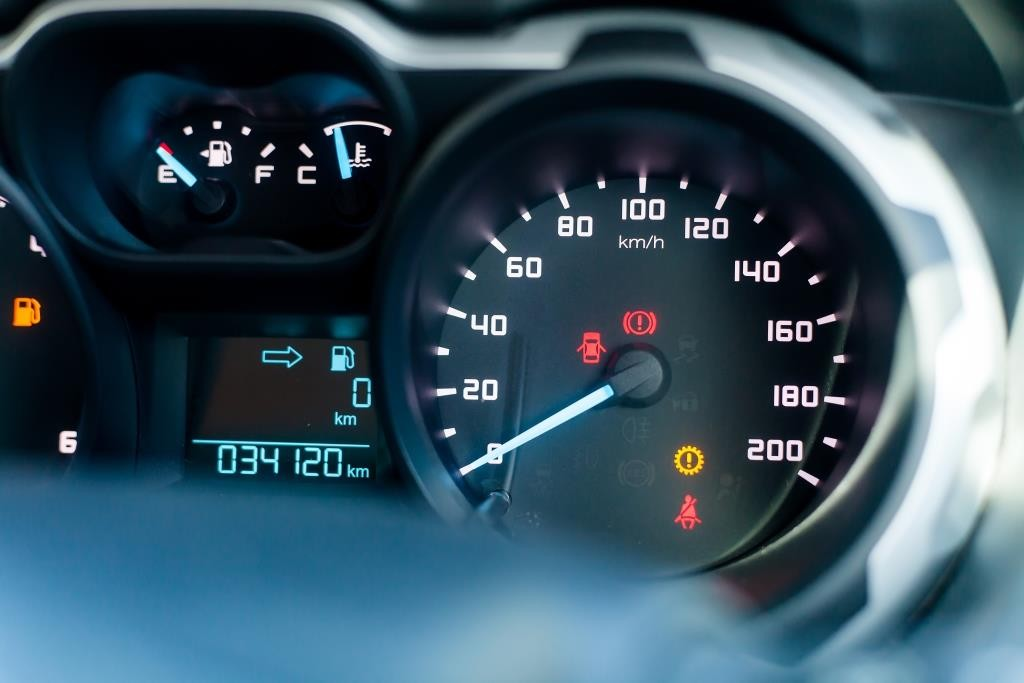
\includegraphics[width=0.7\linewidth]{vitesse_instantanee.png}
    \caption{Un compteur de vitesse indique la vitesse instantanée.}
    \label{vitesse_instantanee}
\end{figure}

\newpage

\subsection{Vecteur vitesse instantanée}
La vitesse instantanée étant définie comme : \(v_{inst}= \lim_{\Delta t \to 0}  \frac{\Delta x}{\Delta t}\), il en découle que le vecteur vitesse instantanée est toujours une \textbf{tangente à la courbe de la position} à l'instant pour lequel on souhaite connaître sa valeur.

\begin{encadre}
    De même, en physique, une vitesse est toujours définie comme étant la \motcle{dérivée de la position par rapport au temps}.
\end{encadre}

\begin{figure}[!ht]
    \centering
    \resizebox{0.8\linewidth}{!}{\begin{tikzpicture}
\definecolor{olivegreen}{RGB} {0,125,15}
\tikzset{>=latex}

\tkzInit[xmin=0,xmax=10,ymin=0,ymax=5,xstep=1,ystep=1]

\tkzDrawX[label={$X [m]$},below left=25pt]
\tkzDrawY[label={$Y [m]$},right=5pt]
\tkzAxeXY[label={}] %This macro combines the four macros: \tkzDrawX\tkzDrawY \tkzLabelX\tkzLabelYnode font=\tiny]

\tkzFct[domain=0:10,red]{(0.1*((0.75*x-4)**3+3*(0.5*x-4)**2+(0.8*x)-4))+2}

\tkzDrawTangentLine[kl=0,kr=1,draw,color=olivegreen](1)
\tkzDrawTangentLine[kl=0,kr=1,draw,color=olivegreen](5)
\tkzDrawTangentLine[kl=0,kr=1,draw,color=olivegreen](8)
\tkzText[color=olivegreen](1.25,2.75){$\vec{v}$}
\tkzText[color=olivegreen](5.5,2){$\vec{v}$}
\tkzText[color=olivegreen](8.5,3){$\vec{v}$}
\end{tikzpicture} 
}
    \caption{Le vecteur vitesse instantanée est toujours tangent à la courbe de la trajectoire.}
    \label{vecteur_vitesse_instantanee}
\end{figure}
\newpage

\subsection{Application}
À partir du graphique ci-dessous :
\begin{enumerate}
    \item complète le tableau \\
          \renewcommand{\arraystretch}{1.5}
          \begin{tabularx}{.8\linewidth}{|X|X|}
              \hline
              Temps [s] & Position [m] \\
              \hline
                        &              \\
              \hline
                        &              \\
              \hline
                        &              \\
              \hline
                        &              \\
              \hline
                        &              \\
              \hline
          \end{tabularx}
          \renewcommand{\arraystretch}{1}
          \\
    \item calcule la vitesse moyenne entre la position O et A \dotfill
    \item calcule la vitesse moyenne entre la position A et B \dotfill
    \item calcule la vitesse moyenne entre la position B et C \dotfill
    \item calcule la vitesse moyenne entre la position O et C \dotfill
    \item calcule la vitesse moyenne entre la position A et D \dotfill
    \item Que peux-tu en conclure? \dotfill \\
          . \dotfill \\
          . \dotfill \\
          . \dotfill
    \item calcule la vitesse moyenne entre la position O et D \dotfill
\end{enumerate}

\newpage
\begin{figure}[!ht]
    \centering
    \resizebox{\linewidth}{!}{\begin{tikzpicture}[>=latex]

\definecolor{majorgrid_gray}{RGB} {192,192,192}
\definecolor{minorgrid_gray}{RGB} {232,232,232}
%\definecolor{my_orange}{RGB} {255,192,120}

\def\tkzCoeffSubColor{20} 
\def\tkzCoeffSubLw{0.2}

\tkzInit[xmax=22,ymax=14,xstep=1,ystep=1]
\tkzGrid[color=majorgrid_gray,line width=0.2mm,sub,subxstep=.5,subystep=.5]

%\tkzText[rotate=90](-1,7){$Position[m]$}
%\tkzText(11,-1){$Temps[s]$}
\tkzDrawX[label={$Temps[s]$},below left=25pt]
\tkzDrawY[label={$Position[m]$},right=5pt]
\tkzAxeXY[label={}] %This macro combines the four macros: \tkzDrawX\tkzDrawY \tkzLabelX\tkzLabelY
 
\tkzDefPoints{0/0/O, 5/6/A, 13/6/B, 16/14/C, 21/0/D};
\tkzDrawSegments[color=black](O,A A,B B,C C,D);
\tkzDrawPoints[color=blue](O,A,B,C,D);
\tkzLabelPoints[above right,color=blue](A,B,C,D);
\tkzLabelPoint[above right,color=blue](O){O};
\end{tikzpicture}

}
    \caption{Le graphique de la position en fonction du temps.}
    \label{exercice_deplacement_1}
\end{figure}

\newpage

\subsection{Applications}
\begin{enumerate}
    \item Le graphique ci-dessous représente la trajectoire d'un mobile. Représente l'allure du vecteur vitesse à différents moments de ce mouvement.
          \begin{figure}[!ht]
              \centering
              \resizebox{.8\linewidth}{!}{\begin{tikzpicture}

\tkzInit[xmin=0,xmax=10,ymin=0,ymax=5,xstep=1,ystep=1]

\tkzDrawX[label={$X [m]$},below left=25pt]
\tkzDrawY[label={$Y [m]$},right=5pt]
\tkzAxeXY[label={}] %This macro combines the four macros: \tkzDrawX\tkzDrawY \tkzLabelX\tkzLabelYnode font=\tiny]

\tkzFct[domain=0:10,red]{-0.01*(x-6)**4+0.3*(x-6)**2+2}

\end{tikzpicture} 
}
              \caption{Le graphique de la trajectoire.}
              \label{exercice_deplacement_2}
          \end{figure}
    \item Un mobile se déplace vers l'Est à la vitesse de \(\num{3} \unit{[m/s]}\) durant \(12 \unit{[s]}\). Il s'arrête puis repart vers le Nord-Ouest à la vitesse \(2 \sqrt{2} \unit{[m/s]}\) durant \(6\unit{[s]}\).
          \begin{enumerate}[label=\alph*)]
              \item Quelle est la longueur totale de la trajectoire ?
              \item Quelle est la longueur du déplacement horizontal ?
              \item Quelle est la longueur du déplacement vertical ?
              \item Quelle est la longueur du déplacement total ?
          \end{enumerate}
\end{enumerate}

